\chapter{MANO Scalability}
\label{ch:Scalability}

In this chapter we discuss the two directions we explored to investigate MANO orchestrator scalability. First, we discuss the scalability plugin that was added to pishahang. The scalability plugin adds 3 main functionalities to pishahang, 1) spawn new child instances of pishahang by allocating new physical resources, 2) Redirecting requests from parent MANO to the child instances and 3) managing the state of child instances. Second, we discuss the experiments conducted on OSM and Pishahang to understand the resource utilization. We also propose a more generic framework to characterize and analyze MANO under load.

\section{Introduction}

\todo[inline]{Add content}

\subsection{Definition of scaling}
`Scalability' is defined in different ways in various academic work. Some of the definitions are listed below.
\begin{itemize}	 
	
	\item "The ability of a particular system to fit a problem as the scope of that problem increases (number of elements or objects, growing volumes of work and/or being susceptible to enlargement)." \cite{furht_handbook_2010}
	
	\item "Scalability of service is a desirable property of a service which provides an ability to handle growing amounts of service loads without suffering significant degradation in relevant quality attributes. The scalability enhanced by scalability assuring schemes such as adding various resources should be proportional to the cost to apply the schemes." \cite{lee_software_2010}
	
	\item "Scalability is the ability of an application to be scaled up to meet demand through replication and distribution of requests across a pool or farm of servers." \cite{chieu_scalability_2011}
	
	\item "A system is said to be scalable if it can handle the addition of users and resources without suffering a noticeable loss of performance or increase in administrative complexity" \cite{noauthor_scale_nodate}
	
\end{itemize}

\subsection{Why does a MANO need scaling?}
\paragraph{}
In recent years, distributed systems have gained an increase in the number of users and resources. Scaling such a system is an important aspect when large user requests have to be served without compromising system performance or increase in administrative complexity. In terms of MANO, when there are a large number Network Service(NS) instantiation of various network functions, they need to be instantiated considering all the relevant metrics of the system.

\paragraph{System load:}
In a distributed system, the system load is the large amount of data that is to be managed by network services increasing the total number of requests for service.
The load on a MANO can be defined in terms of it's load on NFV Orchestrator (NFVO) to process large number of tasks like on-boarding, instantiation and monitoring of VNFs. The NFVO of a MANO receives monitoring information which also increases the load on NFVO triggering it to scale the network service across multiple MANOs in a distributed system \cite{soenen2017optimising}.


\paragraph{Lifecycle Management \& service provisioning:} To provision a network service, the NFVO of a MANO's functionality include instantiation, global resource management scaling in/out , event correlation and termination of services. These functionalities form the lifecycle of NS. With the increase in instantiation of NS over a distributed network, the lifecycle management of each service is a overhead, hence increasing the provision time. This can be better handled when the MANO can be scaled out. To manage services with a closer proximity of geographical region, MANOs could be scaled in.



\section{Scalability Plugin}

\subsection{Introduction}
\subsection{Architecture}
\subsection{Workflow}

\section{Experiments}
\todo[inline]{In this section, only talk about the 180 experiment that gave te horizontal graphs}

\subsection{Idea}
\todo[inline]{Here, talk about the idea behind running the experiment and getting to know the docker containers that took the most resources}

\subsection{Testbed}
\todo[inline]{Explain about the machine configuration used to run the experiments, what OS, how many servers and what VIMs where installed, what is the configuration and how python-mano-wrappers were used to send the requests. }

\todo[inline]{Basically explain the whole experiment setup that was used to conduct the experiment.}

\subsection{OSM Results}
\todo[inline]{OSM Just like you did in the presentation, explain the functionalities of the top 5 dockers and why they are taking}

\subsubsection{CPU}

\begin{figure}[h]
	\centering
	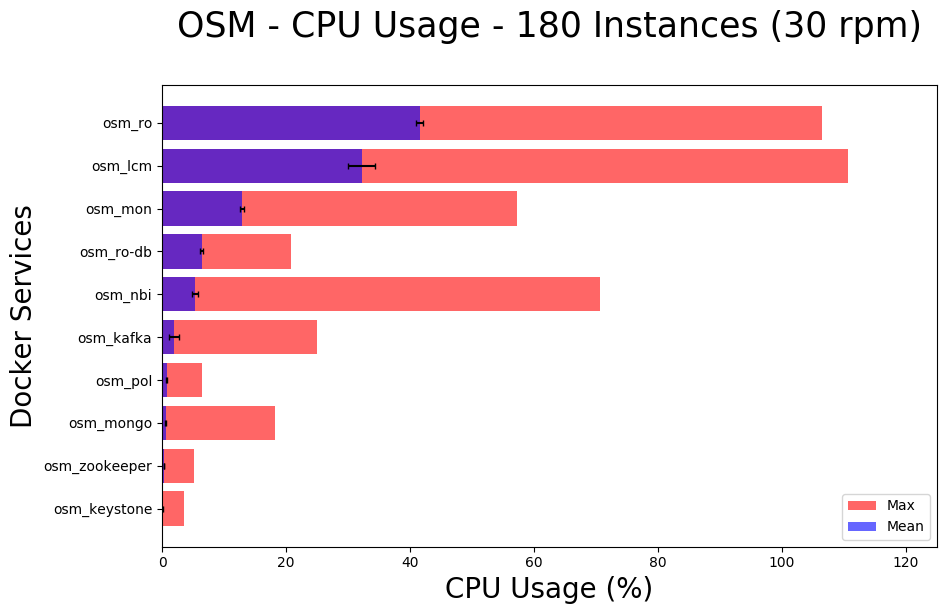
\includegraphics[width=0.7\linewidth]{../figures/scalability_graphs/Horizontal-Docker-Graphs/osm/cirros_case1_180-CPU}
	\caption{OSM CPU}
	\label{fig:cirroscase1180-cpu}
\end{figure}

\subsubsection{Memory}

\begin{figure}[h]
	\centering
	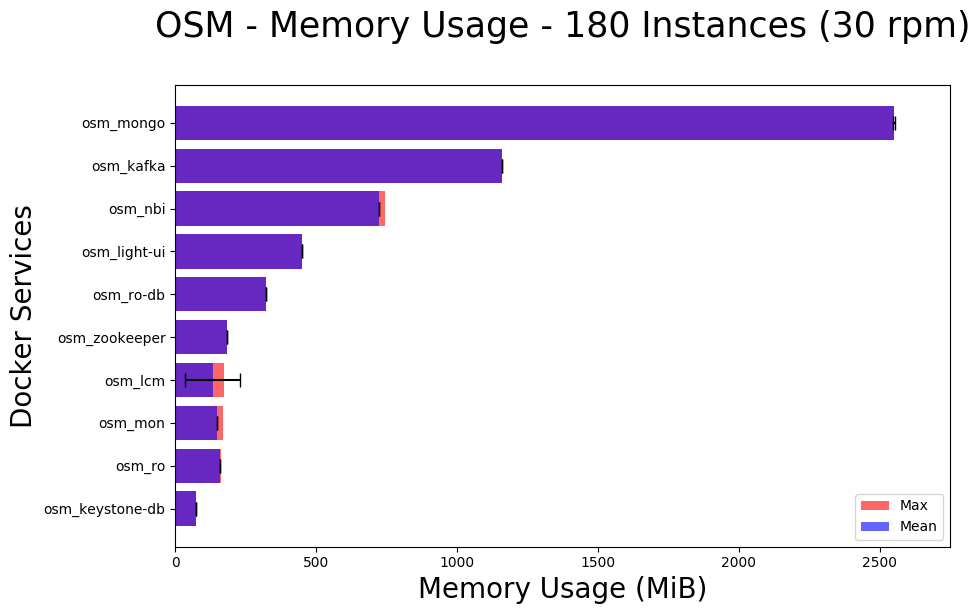
\includegraphics[width=0.7\linewidth]{../figures/scalability_graphs/Horizontal-Docker-Graphs/osm/cirros_case1_180-MEM}
	\caption{OSM MEM}
	\label{fig:cirroscase1180-mem}
\end{figure}

\subsubsection{Lifecycle}

\begin{figure}[h]
	\centering
	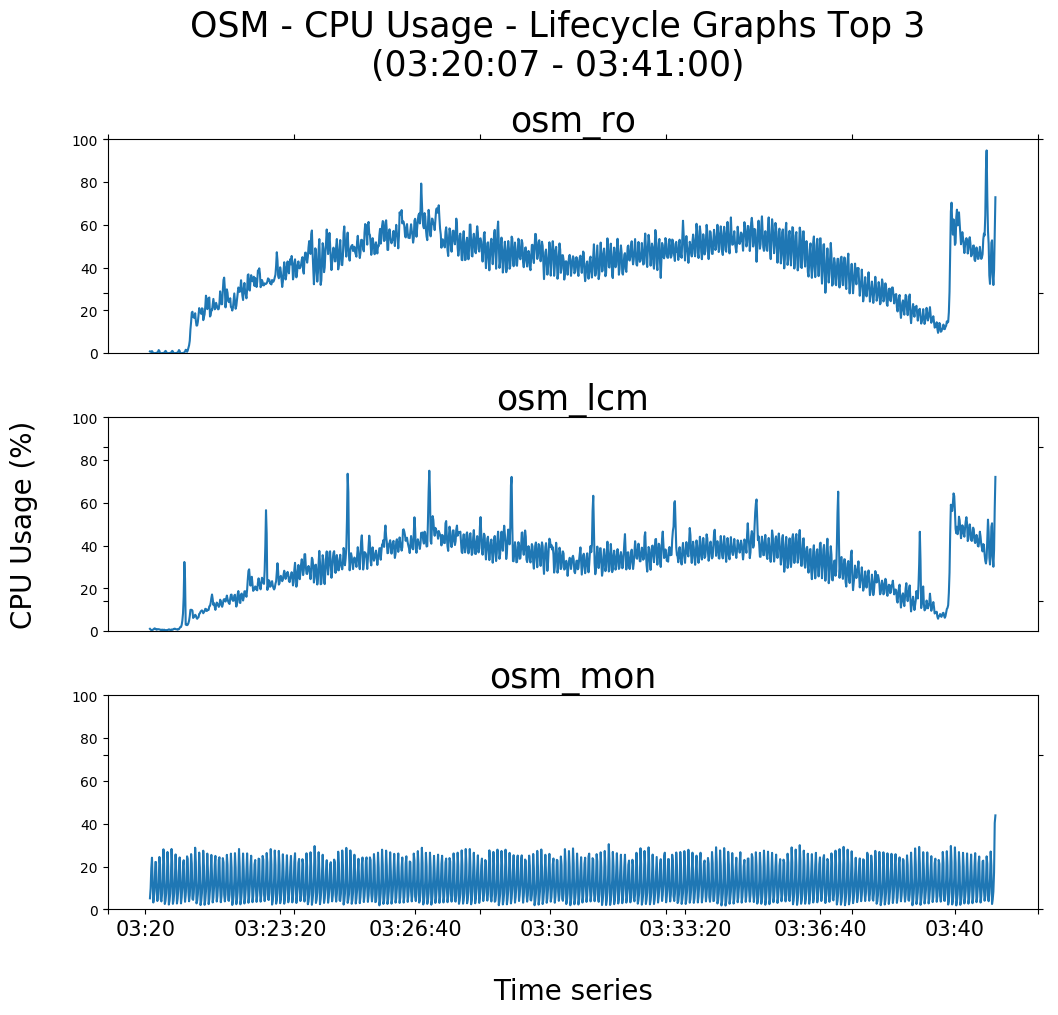
\includegraphics[width=0.7\linewidth]{figures/scalability_graphs/Lifecycle-Graphs-Top-3/OSM-TOP-3-Lifecycle}
	\caption{OSM LS}
	\label{fig:osm-top-3-lifecycle}
\end{figure}


\subsection{Pishahang Results}
\todo[inline]{Pishahang Just like you did in the presentation, explain the functionalities of the top 5 dockers and why they are taking}

\subsubsection{CPU}

\begin{figure}[h]
	\centering
	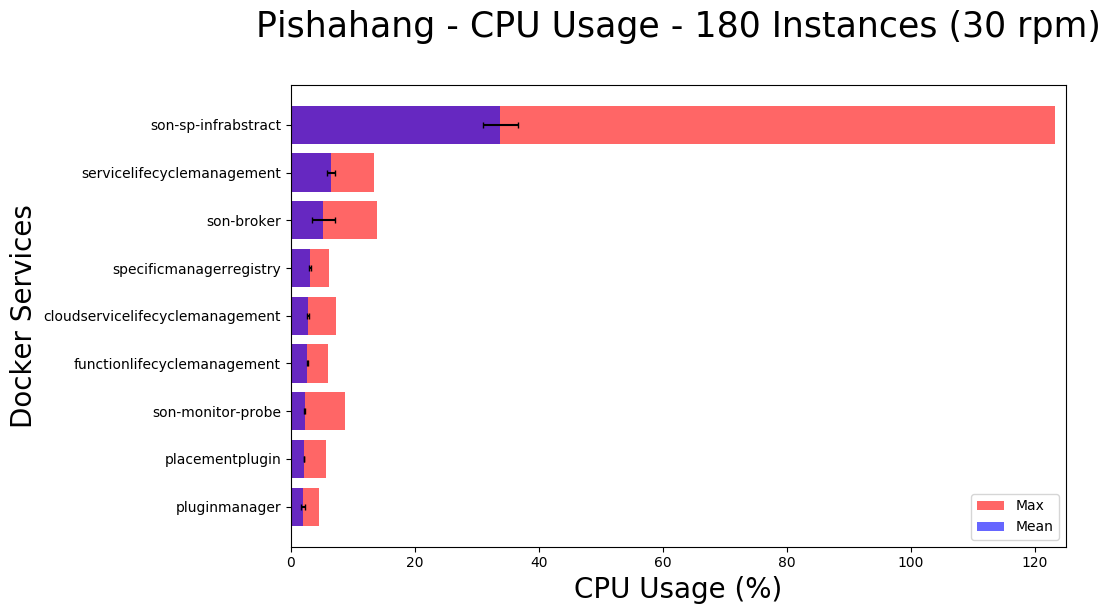
\includegraphics[width=0.7\linewidth]{../figures/scalability_graphs/Horizontal-Docker-Graphs/pishahang/cirros_case1_180-CPU}
	\caption{Pishahang CPU}
	\label{fig:cirroscase1180-cpu}
\end{figure}

\subsubsection{Memory}

\begin{figure}[h]
	\centering
	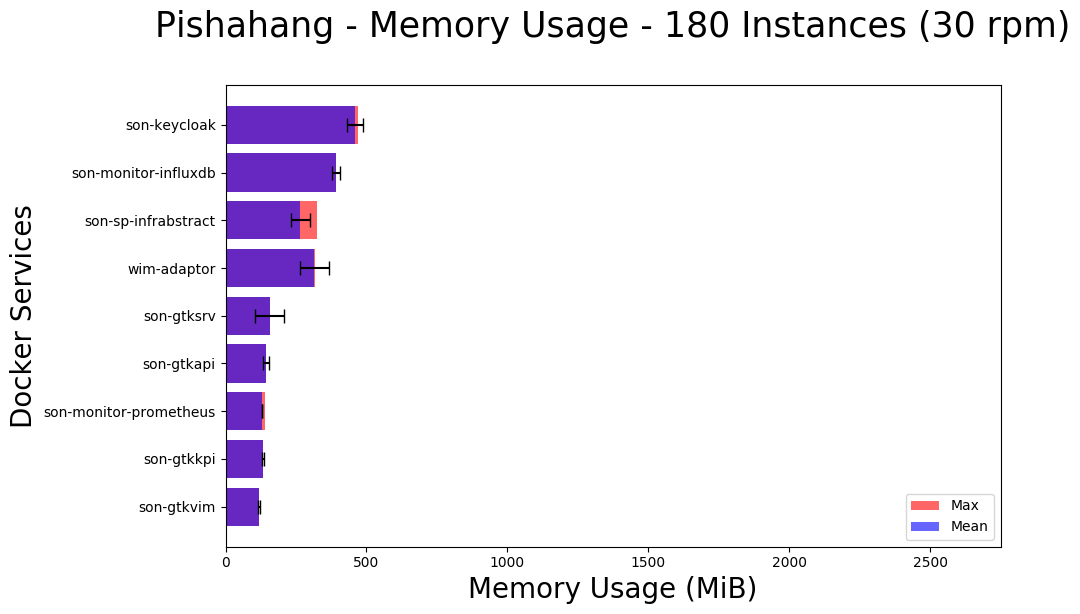
\includegraphics[width=0.7\linewidth]{../figures/scalability_graphs/Horizontal-Docker-Graphs/pishahang/cirros_case1_180-MEM}
	\caption{Pishahang MEM}
	\label{fig:cirroscase1180-mem}
\end{figure}


\subsubsection{Lifecycle}

\begin{figure}[h]
	\centering
	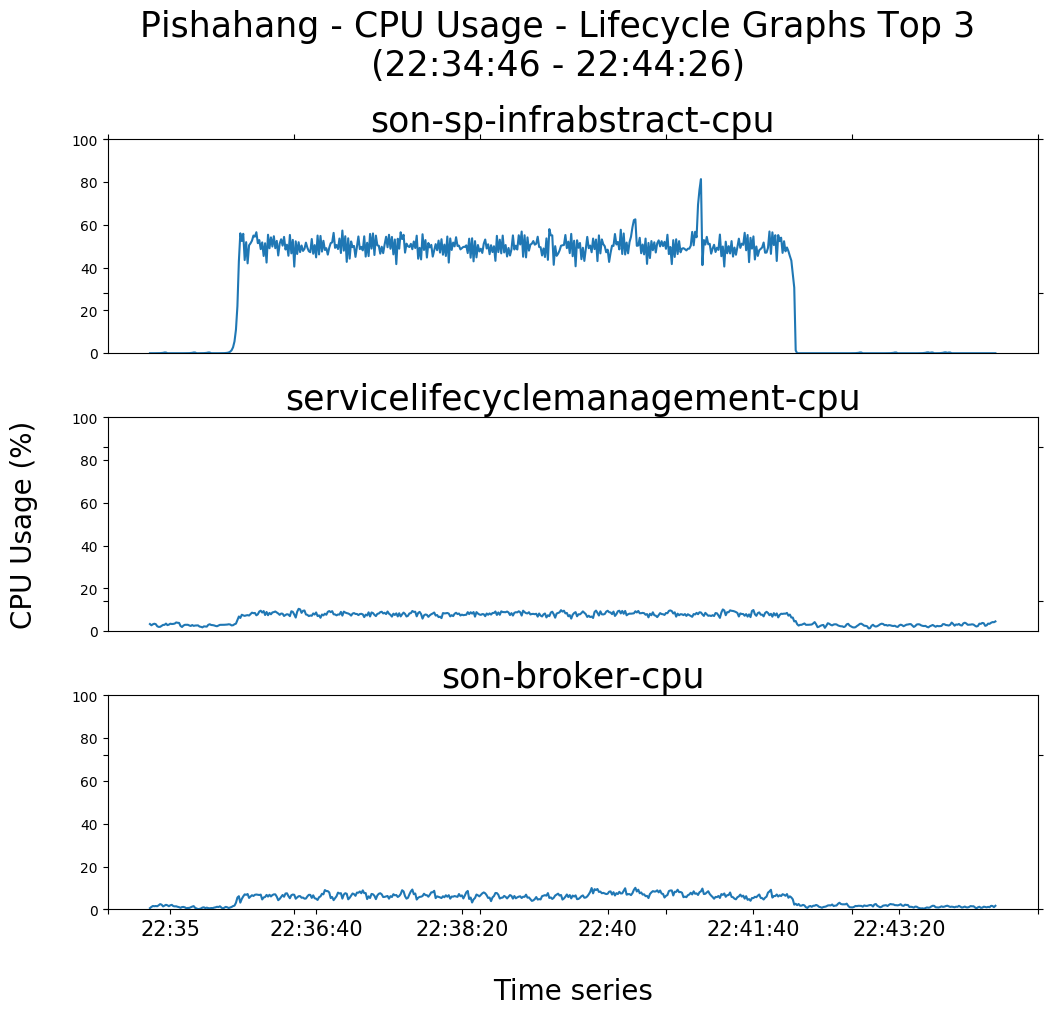
\includegraphics[width=0.7\linewidth]{figures/scalability_graphs/Lifecycle-Graphs-Top-3/Pishahang-TOP-3-Lifecycle}
	\caption{Pish LS}
	\label{fig:pishahang-top-3-lifecycle}
\end{figure}

\subsection{Summary of issues of the experiment}
\todo[inline]{Blockers: VIM support issues, openstack not stable, k8 not supported in OSM. Why 180. RPM issues}
	
\subsection{Inference from the experiment} 
\todo[inline]{about identifying the top dockers, some more info about the lifecycle graphs}

\section{MANO Benchmarking Framework} 

\subsection{Introduction}
\todo[inline]{High level explanation}

\subsection{Design}
\todo[inline]{Explain tools and other techs used}

\subsection{Parameters and KPIs} 
\todo[inline]{Explain the variable parameters and possible KPIs from the experiments}

\subsection{Steps for the automated experiment run} 
\todo[inline]{A walkthrough of the experiment runner}

\subsection{Example Use Cases}
\todo[inline]{Explain results acquired from MANO benchmarking tool}

\subsubsection{Comparison of different network services} 

Comparison of different network services

\begin{figure}[h]
	\centering
	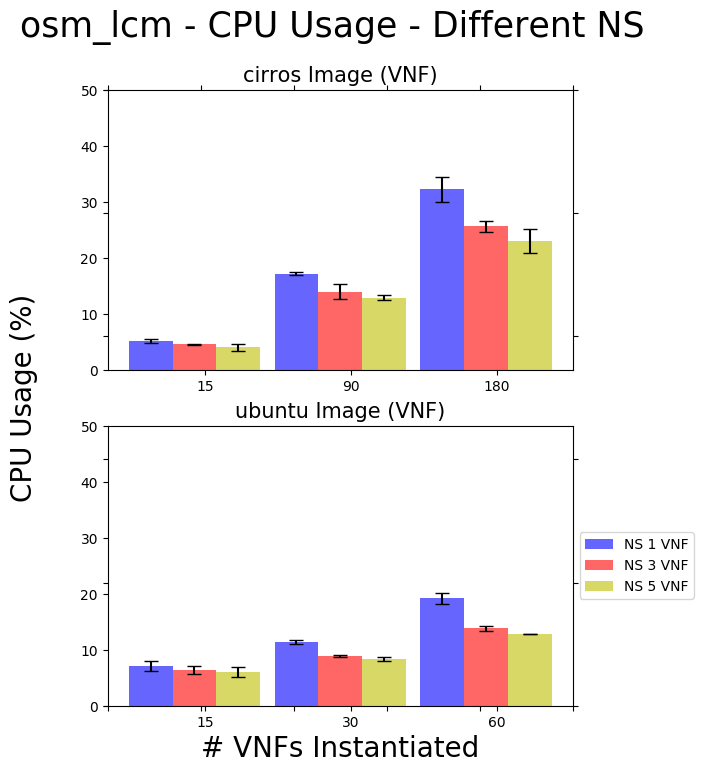
\includegraphics[width=0.7\linewidth]{figures/scalability_graphs/Docker-Grouped-Cases/osm/osm_lcm-Mean-CPU-Cases}
	\caption{}
	\label{fig:osmlcm-mean-cpu-cases}
\end{figure}

\begin{figure}[h]
	\centering
	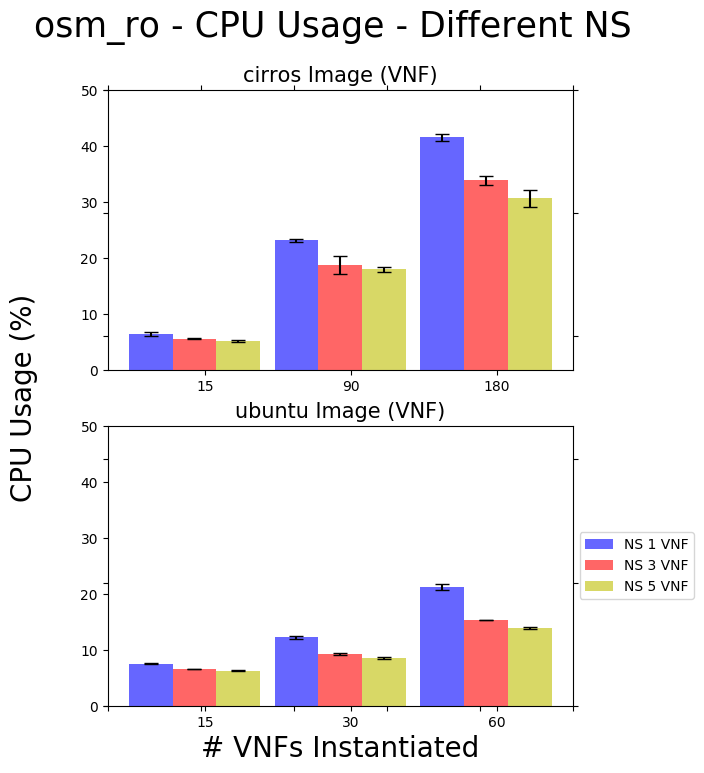
\includegraphics[width=0.7\linewidth]{figures/scalability_graphs/Docker-Grouped-Cases/osm/osm_ro-Mean-CPU-Cases}
	\caption{}
	\label{fig:osmro-mean-cpu-cases}
\end{figure}


\subsubsection{Container vs VM Orchestration} 

Container vs VM Orchestration

\begin{figure}[h]
	\centering
	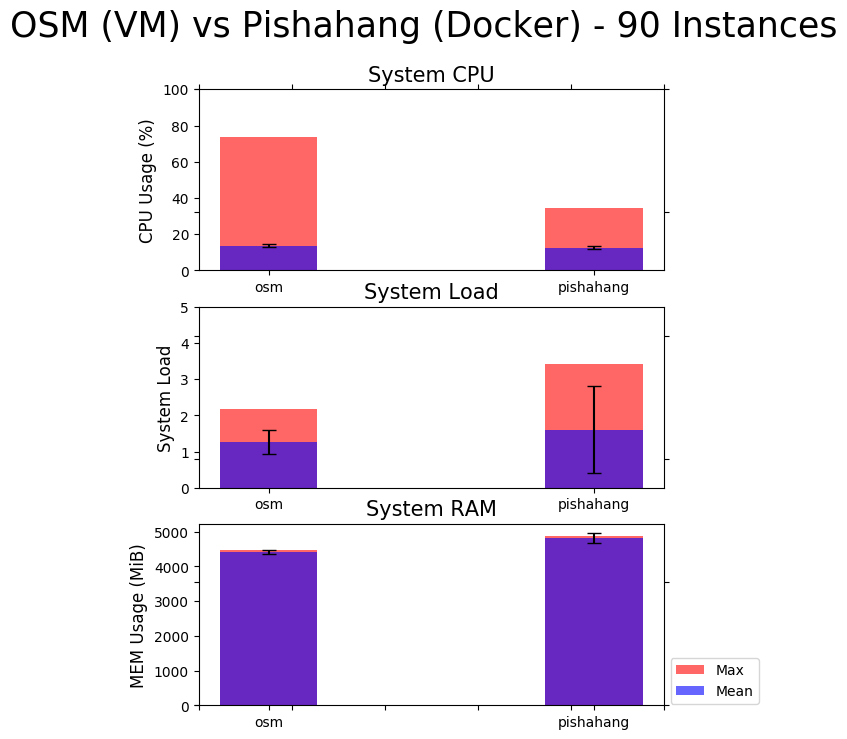
\includegraphics[width=0.7\linewidth]{figures/scalability_graphs/Comparison-VM-Docker/System_metrics_comparison}
	\caption{}
	\label{fig:systemmetricscomparison}
\end{figure}

\begin{figure}[h]
	\centering
	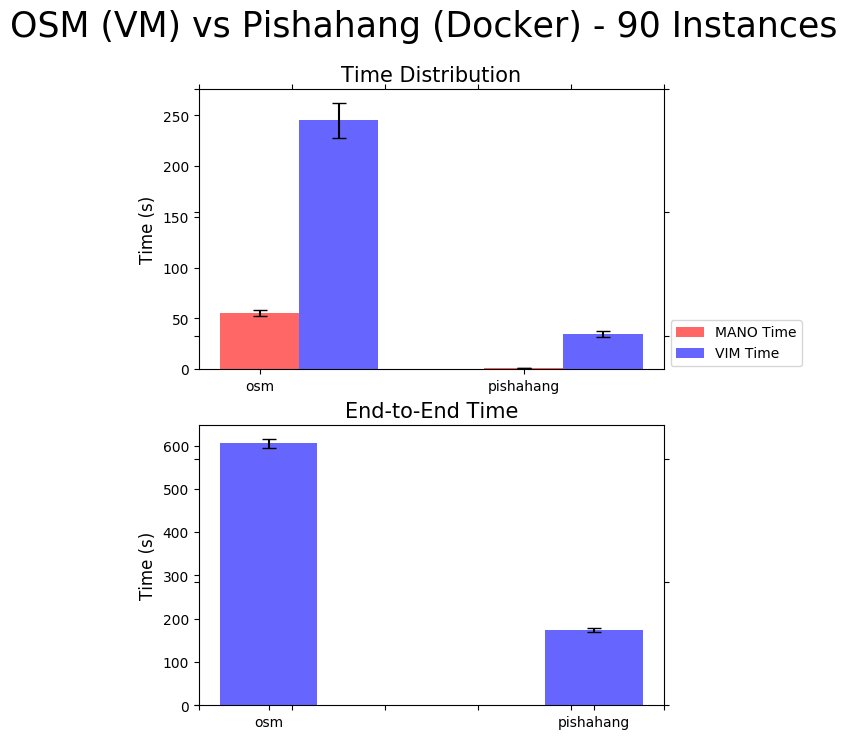
\includegraphics[width=0.7\linewidth]{figures/scalability_graphs/Comparison-VM-Docker/Time_comparison}
	\caption{}
	\label{fig:timecomparison}
\end{figure}


\subsubsection{Scaling Plugin Evaluation}

\begin{figure}[h]
	\centering
	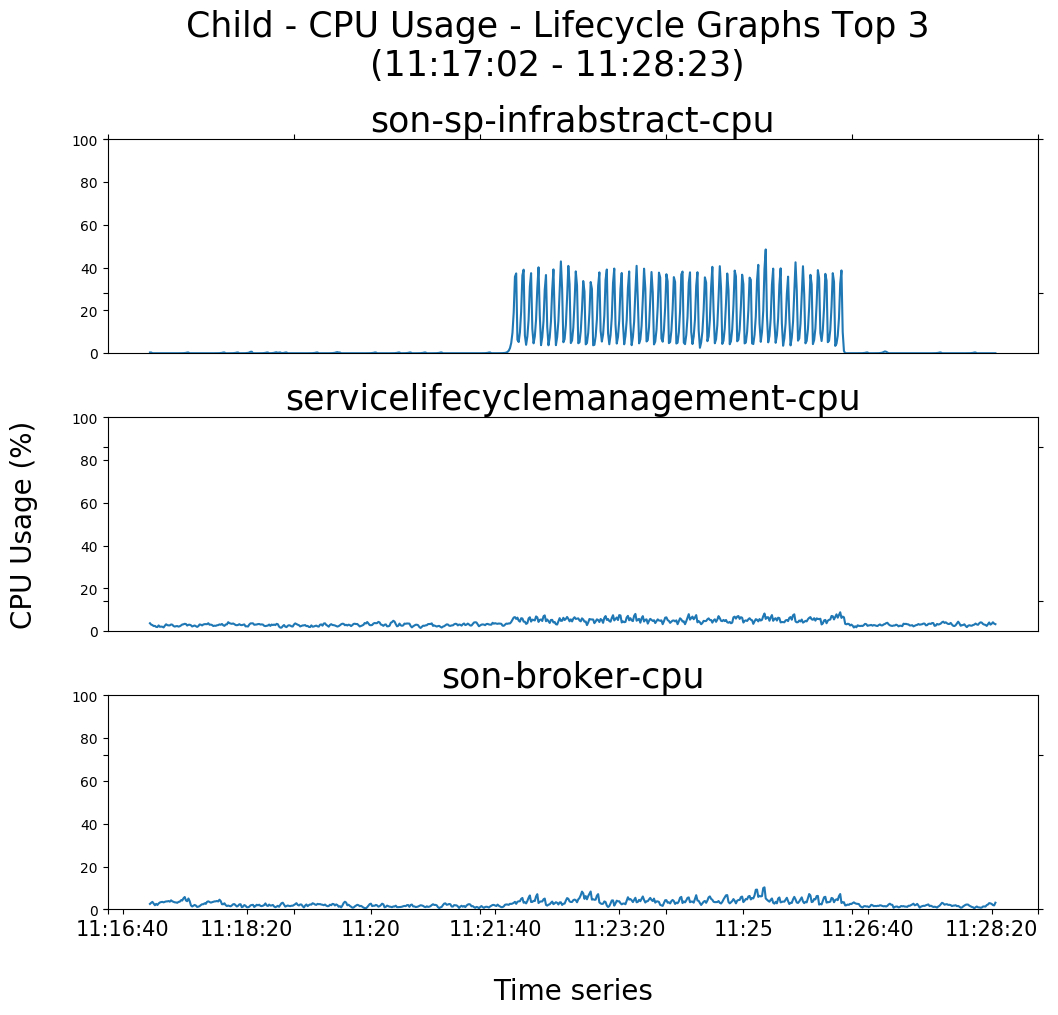
\includegraphics[width=0.7\linewidth]{figures/scalability_graphs/Scalability-Evaluation/Child-TOP-3-Lifecycle}
	\caption{Child scaling}
	\label{fig:child-top-3-lifecycle}
\end{figure}

\begin{figure}[h]
	\centering
	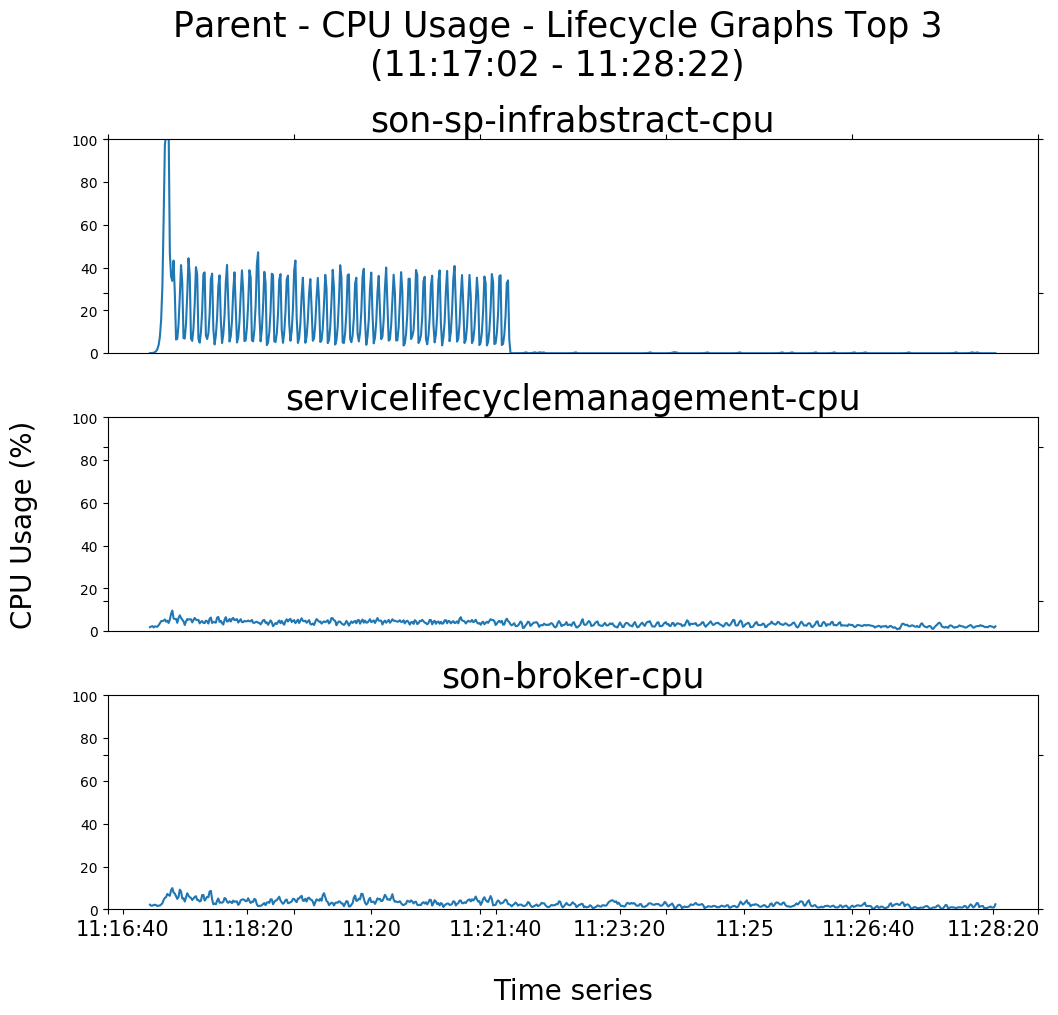
\includegraphics[width=0.7\linewidth]{figures/scalability_graphs/Scalability-Evaluation/Parent-TOP-3-Lifecycle}
	\caption{Parent Scaling}
	\label{fig:parent-top-3-lifecycle}
\end{figure}


\subsection{Future scope}